\documentclass[a4paper,11pt,oneside]{memoir}

% Castellano
\usepackage[spanish,es-tabla]{babel}
\selectlanguage{spanish}
\usepackage[utf8]{inputenc}
\usepackage{placeins}
\usepackage{float}

\RequirePackage{booktabs}
\RequirePackage[table]{xcolor}
\RequirePackage{xtab}
\RequirePackage{multirow}

% Multi-page tables using
\usepackage{longtable}
\usepackage{tabularx}

% Cell with line break (e.g. \specialcell{Foo\\bar})
\newcommand{\specialcell}[2][c]{%
  \begin{tabular}[#1]{@{}l@{}}#2\end{tabular}}

% Mathematic font
\usepackage{amsfonts}

% Color

% Bibliography management
\usepackage[numbers,sort]{natbib}

% Links
\usepackage[colorlinks]{hyperref}
\hypersetup{
	colorlinks,
	linkcolor={green!40!black},
	citecolor={blue!50!black},
	urlcolor={blue!80!black}
}

% Ecuaciones
\usepackage{amsmath}

% Rutas de fichero / paquete
\newcommand{\ruta}[1]{{\sffamily #1}}

% Párrafos
\nonzeroparskip

% Listas estrechas
\providecommand{\tightlist}{%
  \setlength{\itemsep}{0pt}\setlength{\parskip}{0pt}}

% Imagenes
\usepackage{graphicx}
\newcommand{\imagen}[2]{
	\begin{figure}[!h]
		\centering
		\includegraphics[width=0.9\textwidth]{#1}
		\caption{#2}\label{fig:#1}
	\end{figure}
	\FloatBarrier
}

\newcommand{\imagenflotante}[2]{
	\begin{figure}%[!h]
		\centering
		\includegraphics[width=0.9\textwidth]{#1}
		\caption{#2}\label{fig:#1}
	\end{figure}
}



% El comando \figura nos permite insertar figuras comodamente, y utilizando
% siempre el mismo formato. Los parametros son:
% 1 -> Porcentaje del ancho de página que ocupará la figura (de 0 a 1)
% 2 --> Fichero de la imagen
% 3 --> Texto a pie de imagen
% 4 --> Etiqueta (label) para referencias
% 5 --> Opciones que queramos pasarle al \includegraphics
% 6 --> Opciones de posicionamiento a pasarle a \begin{figure}
\newcommand{\figuraConPosicion}[6]{%
  \setlength{\anchoFloat}{#1\textwidth}%
  \addtolength{\anchoFloat}{-4\fboxsep}%
  \setlength{\anchoFigura}{\anchoFloat}%
  \begin{figure}[#6]
    \begin{center}%
      \Ovalbox{%
        \begin{minipage}{\anchoFloat}%
          \begin{center}%
            \includegraphics[width=\anchoFigura,#5]{#2}%
            \caption{#3}%
            \label{#4}%
          \end{center}%
        \end{minipage}
      }%
    \end{center}%
  \end{figure}%
}

%
% Comando para incluir imágenes en formato apaisado (sin marco).
\newcommand{\figuraApaisadaSinMarco}[5]{%
  \begin{figure}%
    \begin{center}%
    \includegraphics[angle=90,height=#1\textheight,#5]{#2}%
    \caption{#3}%
    \label{#4}%
    \end{center}%
  \end{figure}%
}
% Para las tablas
\newcommand{\otoprule}{\midrule [\heavyrulewidth]}
%
% Nuevo comando para tablas pequeñas (menos de una página).
\newcommand{\tablaSmall}[5]{%
 \begin{table}[H]
  \begin{center}
   \rowcolors {2}{gray!35}{}
   \begin{tabular}{#2}
    \toprule
    #4
    \otoprule
    #5
    \bottomrule
   \end{tabular}
   \caption{#1}
   \label{tabla:#3}
  \end{center}
 \end{table}
}

%
% Nuevo comando para tablas pequeñas (menos de una página).
\newcommand{\tablaSmallSinColores}[5]{%
 \begin{table}[H]
  \begin{center}
   \begin{tabular}{#2}
    \toprule
    #4
    \otoprule
    #5
    \bottomrule
   \end{tabular}
   \caption{#1}
   \label{tabla:#3}
  \end{center}
 \end{table}
}

\newcommand{\tablaApaisadaSmall}[5]{%
\begin{landscape}
  \begin{table}
   \begin{center}
    \rowcolors {2}{gray!35}{}
    \begin{tabular}{#2}
     \toprule
     #4
     \otoprule
     #5
     \bottomrule
    \end{tabular}
    \caption{#1}
    \label{tabla:#3}
   \end{center}
  \end{table}
\end{landscape}
}

%
% Nuevo comando para tablas grandes con cabecera y filas alternas coloreadas en gris.
\newcommand{\tabla}[6]{%
  \begin{center}
    \tablefirsthead{
      \toprule
      #5
      \otoprule
    }
    \tablehead{
      \multicolumn{#3}{l}{\small\sl continúa desde la página anterior}\\
      \toprule
      #5
      \otoprule
    }
    \tabletail{
      \hline
      \multicolumn{#3}{r}{\small\sl continúa en la página siguiente}\\
    }
    \tablelasttail{
      \hline
    }
    \bottomcaption{#1}
    \rowcolors {2}{gray!35}{}
    \begin{xtabular}{#2}
      #6
      \bottomrule
    \end{xtabular}
    \label{tabla:#4}
  \end{center}
}

%
% Nuevo comando para tablas grandes con cabecera.
\newcommand{\tablaSinColores}[6]{%
  \begin{center}
    \tablefirsthead{
      \toprule
      #5
      \otoprule
    }
    \tablehead{
      \multicolumn{#3}{l}{\small\sl continúa desde la página anterior}\\
      \toprule
      #5
      \otoprule
    }
    \tabletail{
      \hline
      \multicolumn{#3}{r}{\small\sl continúa en la página siguiente}\\
    }
    \tablelasttail{
      \hline
    }
    \bottomcaption{#1}
    \begin{xtabular}{#2}
      #6
      \bottomrule
    \end{xtabular}
    \label{tabla:#4}
  \end{center}
}

%
% Nuevo comando para tablas grandes sin cabecera.
\newcommand{\tablaSinCabecera}[5]{%
  \begin{center}
    \tablefirsthead{
      \toprule
    }
    \tablehead{
      \multicolumn{#3}{l}{\small\sl continúa desde la página anterior}\\
      \hline
    }
    \tabletail{
      \hline
      \multicolumn{#3}{r}{\small\sl continúa en la página siguiente}\\
    }
    \tablelasttail{
      \hline
    }
    \bottomcaption{#1}
  \begin{xtabular}{#2}
    #5
   \bottomrule
  \end{xtabular}
  \label{tabla:#4}
  \end{center}
}



\definecolor{cgoLight}{HTML}{EEEEEE}
\definecolor{cgoExtralight}{HTML}{FFFFFF}

%
% Nuevo comando para tablas grandes sin cabecera.
\newcommand{\tablaSinCabeceraConBandas}[5]{%
  \begin{center}
    \tablefirsthead{
      \toprule
    }
    \tablehead{
      \multicolumn{#3}{l}{\small\sl continúa desde la página anterior}\\
      \hline
    }
    \tabletail{
      \hline
      \multicolumn{#3}{r}{\small\sl continúa en la página siguiente}\\
    }
    \tablelasttail{
      \hline
    }
    \bottomcaption{#1}
    \rowcolors[]{1}{cgoExtralight}{cgoLight}

  \begin{xtabular}{#2}
    #5
   \bottomrule
  \end{xtabular}
  \label{tabla:#4}
  \end{center}
}


















\graphicspath{ {../img/} }

% Capítulos
\chapterstyle{bianchi}
\newcommand{\capitulo}[2]{
	\setcounter{chapter}{#1}
	\setcounter{section}{0}
	\chapter*{#2}
	\addcontentsline{toc}{chapter}{#2}
	\markboth{#2}{#2}
}

% Apéndices
\renewcommand{\appendixname}{Apéndice}
\renewcommand*\cftappendixname{\appendixname}

\newcommand{\apendice}[1]{
	%\renewcommand{\thechapter}{A}
	\chapter{#1}
}

\renewcommand*\cftappendixname{\appendixname\ }

% Formato de portada
\makeatletter
\usepackage{xcolor}
\newcommand{\tutor}[1]{\def\@tutor{#1}}
\newcommand{\course}[1]{\def\@course{#1}}
\definecolor{cpardoBox}{HTML}{E6E6FF}
\def\maketitle{
  \null
  \thispagestyle{empty}
  % Cabecera ----------------
\noindent
\includegraphics[width=\textwidth]{cabecera}\vspace{1cm}%
  \vfill
  % Título proyecto y escudo informática ----------------
  \colorbox{cpardoBox}{%
    \begin{minipage}{.8\textwidth}
      \vspace{.5cm}\Large
      \begin{center}
      \textbf{TFG del Grado en Ingeniería Informática}\vspace{.6cm}\\
      \textbf{\LARGE\@title{}}
      \end{center}
      \vspace{.2cm}
    \end{minipage}

  }%
  \hfill\begin{minipage}{.20\textwidth}
    
\includegraphics[width=\textwidth]{escudoInfor}
  \end{minipage}
  \vfill
  % Datos de alumno, curso y tutores ------------------
  \begin{center}%
  {%
    \noindent\LARGE
    Presentado por \@author{}\\ 
    en la Universidad de Burgos --- \@date{}\\
    Tutores: \@tutor{}\\
  }%
  \end{center}%
  \null
  \cleardoublepage
  }
\makeatother

\newcommand{\nombre}{David Miguel Lozano} %%% cambio de comando

% Datos de portada
\title{{\Huge GoBees}\\[0.5cm]Monitorización del estado de una colmena mediante la cámara de un smartphone.}
\author{\nombre}
\tutor{Dr. José Francisco Díez Pastor\\y Dr. Raúl Marticorena Sánchez}
\date{\today}

\begin{document}

\maketitle



\newpage\null\thispagestyle{empty}\newpage


%%%%%%%%%%%%%%%%%%%%%%%%%%%%%%%%%%%%%%%%%%%%%%%%%%%%%%%%%%%%%%%%%%%%%%%%%%%%%%%%%%%%%%%%
\thispagestyle{empty}


\noindent
\includegraphics[width=\textwidth]{cabecera}\vspace{1cm}

\noindent D. José Francisco Díez Pastor y D. Raúl Marticorena Sánchez, profesores del departamento de Ingeniería Civil, área de Lenguajes y Sistemas Informáticos.

\noindent Exponen:

\noindent Que el alumno D. \nombre, con DNI 71307412Y, ha realizado el Trabajo Final de Grado en Ingeniería Informática titulado ``GoBees - Monitorización del estado de una colmena mediante la cámara de un smartphone''. 

\noindent Y que dicho trabajo ha sido realizado por el alumno bajo la dirección del que suscribe, en virtud de lo cual se autoriza su presentación y defensa.

\begin{center} %\large
En Burgos, {\large \today}
\end{center}

\vfill\vfill\vfill

% Author and supervisor
\begin{minipage}{0.45\textwidth}
\begin{flushleft} %\large
Vº. Bº. del Tutor:\\[2cm]
D. José Francisco Díez Pastor
\end{flushleft}
\end{minipage}
\hfill
\begin{minipage}{0.45\textwidth}
\begin{flushleft} %\large
Vº. Bº. del Tutor:\\[2cm]
D. Raúl Marticorena Sánchez
\end{flushleft}
\end{minipage}
\hfill

\vfill

% para casos con solo un tutor comentar lo anterior
% y descomentar lo siguiente
%Vº. Bº. del Tutor:\\[2cm]
%D. nombre tutor


\newpage\null\thispagestyle{empty}\newpage




\frontmatter

% Abstract en castellano
\renewcommand*\abstractname{Resumen}
\begin{abstract}
La actividad de vuelo de una colmena es un indicador importante sobre su
estado de salud. Sin embargo, la monitorización manual de este parámetro
es un proceso muy costoso y puede introducir una tasa de error elevada.
Por ello, se han desarrollado diversos métodos que permiten automatizar
este proceso.

En este trabajo se propone un nuevo método más accesible al público
general que permite la monitorización de la actividad de vuelo de una
colmena mediante la cámara de un \emph{smartphone} Android.

Además, se ha desarrollado una aplicación de gestión de colmenares que
integra el algoritmo y proporciona las herramientas necesarias para
interpretar y organizar toda la información recabada.

GoBees es la aplicación resultante y se encuentra disponible a través de
Google Play o de la página oficial del proyecto \url{http://gobees.io/}.
\end{abstract}

\renewcommand*\abstractname{Descriptores}
\begin{abstract}
Contador de abejas, actividad de vuelo, monitorización de colmenas, 
gestión de colmenares, aplicación Android.
\end{abstract}

\clearpage

% Abstract en inglés
\renewcommand*\abstractname{Abstract}
\begin{abstract}
Flight activity of a honey bee colony is an overall indicator of the
state of the hive's health. However, manually monitoring this parameter
is a very expensive and time-consuming process and can introduce a high
error rate. Thus, several methods to automate this process have been
developed over the years.

In this work, we propose a new method more accessible to the general
public which allows monitoring the flight activity of a honey bee colony
using the built-in camera of an Android smartphone.

In addition, an apiary management application has been developed,
incorporating the algorithm and providing the necessary tools to
interpret and organize all the information gathered.

GoBees is the resulting application and it is available on Google Play
or the official web site \url{http://gobees.io/}.
\end{abstract}

\renewcommand*\abstractname{Keywords}
\begin{abstract}
Bee counter, flight activity, hive monitoring, apiary management, 
Android application.
\end{abstract}

\clearpage

% Indices
\tableofcontents

\clearpage

\listoffigures

\clearpage

%\listoftables

%\clearpage

\mainmatter
\capitulo{1}{Introducción}

Descripción del contenido del trabajo y del estrucutra de la memoria y del resto de materiales entregados.

\capitulo{2}{Objetivos del proyecto}

%% Comentario de la plantilla
%%Este apartado explica de forma precisa y concisa cuales son los objetivos que se persiguen con la realización del proyecto. Se puede distinguir entre los objetivos marcados por los requisitos del software a construir y los objetivos de carácter técnico que plantea a la hora de llevar a la práctica el proyecto.

A continuación, se detallarán los objetivos que han motivado la realización de este proyecto así como los resultados que se desean conseguir.

\section{Objetivos generales}
\begin{itemize}
	\item Desarrollar una aplicación para \emph{smartphone}.
	\item Implemenación y despliegue de la aplicación en la tienda de apps.
	\item Hacer que los usuarios pasen un buen rato.
\end{itemize}

\section{Objetivos técnicos}
\begin{itemize}
	\item Aprender una alternativa moderna a javascript mediante Dart.
	\item Comprender el funcionamiento de Flutter.
	\item Control de versiones con la herramienta GitHub, mediante comandos a través de GitBash.
	\item Generar documentación de todo el proceso en \LaTeX.
	\item Realizar una planificación mediante \emph{Scrum} eficiente, mediante la herramienta ZenHub, integrada en GitHub.
	\item Comunicación de la aplicación mediante WebServices.
	
\end{itemize}

\section{Objetivos personales}
\begin{itemize}
	\item Adquirir el conocimiento necesario para desarrollar aplicaciones móviles y multiplataforma.
	\item Aprobar el trabajo de fin de grado.
	\item Estudiar como generar documentación en \LaTeX.
	\item Aprender que sin esfuerzo no hay recompensa.
\end{itemize}
\capitulo{3}{Conceptos teóricos}

El proyecto cubre todo el proceso de creación de la aplicación, desde el diseño, implementación del código, hasta el despliegue de la misma en la \emph{Play Store}. Para ello se ha tenido que realizar un proceso de búsqueda para determinar que herramientas, lenguajes de programación, entornos de desarrollo son los más apropiados para un despliegue ágil.

Todo esto se sitúa en un mercado altamente competitivo, con una gran variabilidad (usuarios, empresas, desarrolladores ...) y con un constante cambio. 

\section{Aplicaciones nativas}
Estas se denominan así porque se desarrollan en el lenguaje nativo de cada uno de los sistemas operativos. Dependiendo de la plataforma en la que se desee crear esta nueva aplicación requerirá conocer un lenguaje de programación y un entorno de desarrollo en concreto. A continuación se muestra una tabla~\ref{table:nativos} con las herramientas y lenguajes nativos:

\begin{table}[H]
	\begin{center}
		\begin{tabular}{ccc}
			\hline
			Sistema Operativo                        & Lenguaje Programación & Entorno \\ \hline
			Android				    & Java      & Android Studio					\\
			iOS			    & Objetive C, Swift       & Xcode						\\ \hline
		\end{tabular}
		\caption{Herramientas y lenguaje nativos}
		\label{table:nativos}
	\end{center}
\end{table}

Las ventajas principales son: están desarrolladas directamente sobre la capa nativa del dispositivo, el rendimiento será óptimo y todas las funcionalidades y características estarán disponibles desde el primer momento.

Entre las desventajas: el elevado coste y mantenimiento, ya que requiere personal más especializado, con mayor tiempo destinado al desarrollo. Pero el mayor inconveniente lo encontramos en que el código nativo de una plataforma no puede ser reutilizado para la otra. Algo que los frameworks actuales están empezando a ofrecer.

\section{Aplicaciones híbridas mediante Framework}
Un framework (término de origen anglosajón: marco de trabajo)~\cite{wiki:framework}, es una estructura conceptual y tecnológica de soporte definido, normalmente por módulos de software concretos, que sirve de base para la organización y el desarrollo de software. Las ventajas que ofrece son varias, entre las que se puede destacar:

\begin{itemize}
	\item \textbf{Único código fuente}: desarrollo de aplicaciones multiplataforma con un único lenguaje, reduciendo los costes de creación, mantenimiento y recursos destinados. Actualmente no todos los frameworks ofrecen esto, pero en la gran mayoría sí que se está integrando, ya que existe una gran lucha por la competitividad.
	\item \textbf{Evita repetición de código:} las partes más usadas, pasan a ser algo del \emph{core} del framework o simplemente que se pueden reutilizar fácilmente. 
	\item \textbf{Uso de buenas prácticas:} están basados en patrones de diseño que nos obligan a usar.
	\item \textbf{Elementos avanzados integrados:} dispone de librerías nativas que ofrecen \emph{Widgets} o funcionalidades de gran calidad, que llevan mucho tiempo implementar, o que la creación de los mismo desde cero, no llegaría a obtener una calidad del mismo nivel.
	\item \textbf{Desarrollo ágil:} por los factores anteriores, podemos centrarnos más en la lógica de negocio de la aplicación que se desea hacer de una manera más rápida y segura.
\end{itemize}

Por lo tanto, es necesario trabajar mediante frameworks, ya que nos garantiza una aplicación de mayor calidad que si la hacemos en código nativo.

\subsection{Opciones disponibles}
En el mercado existen muchos frameworks disponibles para el desarrollo de aplicaciones móviles, por lo que decantarse por uno no es tarea sencilla, ya que cada uno tiene sus pros y contras. En una encuesta realizada a mediados del 2019 en el siguiente foro: Forocohes~\cite{foro:encuesta}, uno de los más recomendados era Flutter, como se puede ver en la imagen~\ref{fig:encuesta}:

\begin{figure}[h]
	\centering
	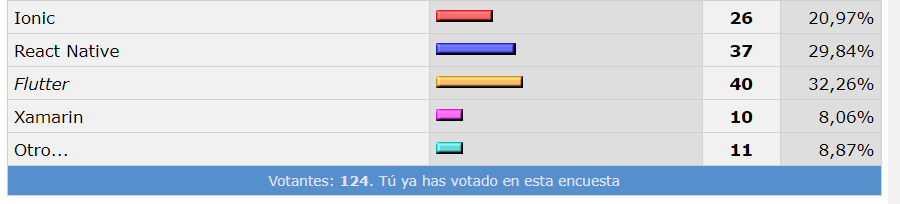
\includegraphics[width=1\textwidth]{teoria/encuesta.png}
	\caption{Encuesta en Forocoches}\label{fig:encuesta}
\end{figure}

Uno de los objetivos a la hora de encontrar el framework con el que hacer la aplicación, es que abarque el mayor número de dispositivos y usuarios. Es decir, que sea un framework \emph{crossplatform} o multiplataforma .

\subsubsection{Ionic}
Ionic~\cite{wiki:ionnic} se basa en lenguaje de programación javascript, html y css. Internamente esta basado en otro framework, como es Angularjs. La licencia es Open source, fue lanzado en el 2013 y permite el desarrollo para iOS y Android. A sufrido gran cantidad de cambios desde entonces.

Ventajas:
\begin{itemize}
	\item Una amplia comunidad de usuarios.
	\item Documentación extensa y de calidad.
\end{itemize}

Algunas de las desventajas:
\begin{itemize}
	\item Rendimiento algo menor, ya que no se desarrolla de forma nativa.
	\item Bibliotecas en constante cambio y evolución, más que ser algo bueno, puede que deje a la aplicación fuera de versión y se tenga que hacer otra vez.
\end{itemize}

\subsubsection{React native}
React native~\cite{wiki:react} fue creado en 2015 de la mano de Facebook. La licencia que tiene es MIT. La diferencia que tiene con React original, es que no manipula el DOM, por lo que tampoco usa HTML o CSS. 
Se programa en javascript. Las aplicaciones más conocidas que usan este framework son Instagram y Facebook.

Ventajas:
\begin{itemize}
	\item Gran comunidad de usuarios y herramientas.
	\item Mejora de las funcionalidades constantemente.
\end{itemize}

Algunas de las desventajas:
\begin{itemize}
	\item Rendimiento algo menor.
	\item No es código nativo, pero casi, por lo que no tiene soporte oficial de Google y Apple.
\end{itemize}

\subsubsection{Xamarin}
Xamarin~\cite{wiki:xamarin} creado por Microsoft en el 2011, por lo que está desarrollado en .NET, siendo propietario.

Ventajas:
\begin{itemize}
	\item Permite el desarrollo de iOS, Android, web y nativas de escritorio.
	\item Puede llamar a fragmentos de código en otros lenguajes usados en otras plataformas.
	\item Soporte para wearables.
\end{itemize}

Algunas de las desventajas:
\begin{itemize}
	\item Acceso limitado a las bibliotecas.
	\item El soporte es escaso y las actualizaciones son poco frecuentes.
	\item Comunidad grande pero pequeña comparada con otras.
	\item Aplicaciones de mayor tamaño.
	\item Mayor coste que otras.
\end{itemize}

\subsubsection{Otros}
Hay muchos otros, como kotlin, Apache Cordoba, jQuery Mobile, Native script...
Pero no me convencieron por diversas razones, como la curva de aprendizaje, costes, dificultades técnicas, entre otras.
 
\section{Flutter}
Flutter~\cite{wiki:flutter} es un SDK de código abierto creado por Google a finales del 2018. Permite que los desarrolladores puedan crear aplicaciones para iOS, Android y web.

Se encuentra escrito en Dart, que es un lenguaje de programación creado por Google en 2011. Pretende conseguir una mejora del lenguaje javascript, pero sin querer sustituirlo. Es decir, ofrecer mejores resultados y alternativas para algunos problemas, siendo una herramienta de mayor calidad para proyectos más grandes y que necesitan un desarrollo veloz.

Flutter es una herramienta muy reciente, con la que se pueden hacer aplicaciones comerciales para varias plataformas sin tener que programar exclusivamente para cada una de ellas. Ya que nos ofrece la compilación nativa directamente, reduciendo los costes a la hora de tener que llevar proyectos en los que sea necesario estar varias plataformas.

Las características más importantes son: 

\begin{itemize}
	\item Desarrollo rápido de las aplicaciones. Cuando se dice rápido es porque permite \emph{hot reload}. Lo que significa carga en caliente durante la fase de desarrollo. Implica que no es necesario tener que compilar todo el código, si no aquellas partes que fueron modificadas. Lo que permite en tiempo de ejecución ver los cambios.
	\item Está muy optimizado, con una evolución y soporte constante.
	\item Es un lenguaje de programación respaldado por Google, con lo que esto conlleva. Seguridad, confianza, fiabilidad, soporte, cursos y un montón de herramientas (más de 300 apis distintas: mapas, reconocimiento facial, traductor ...).
	\item La integración con el sistema operativo Android es mucho más eficaz, ya que este también pertenece a Google.
	\item Cuando se compila lo hace a nativo, ofreciendo una ganancia de rendimiento.
	\item La curva de aprendizaje es baja, en el caso de que sepamos javascript, typescript o ecmascript. Pero en caso contrario, no es especialmente empinada.
	\item La calidad de las animaciones y transiciones.
\end{itemize}

Las desventajas que tiene son:
\begin{itemize}
	\item La mayor parte de la documentación se encuentra en inglés, pero es más problema del desarrollador, que de la propia documentación del framework.
	\item Las aplicaciones ocupan más espacio que las nativas, ya que suelen incluir el SDK al completo.
	\item Al ser tan nuevo, tiene algunos problemas, no ofrece todas las funcionalidades, como las que tienen otras plataformas. Google lo sabe y está trabajando mucho en ello.
	\item Es una comunidad pequeña, pero ha crecido en dos años más que otras en tiempos similares.
\end{itemize}

Al final me decanté por este Framework básicamente porque es algo nuevo y disruptivo. El respaldo de Google se me presentaba como garantía, con la tranquilidad que eso conlleva. Es decir, todo el \emph{cloud services de Google} se puede integrar con gran facilidad.
Otra de las cosas que me incentivaron a elegirlo es que la comunidad lo a recibido con los brazos abiertos, como se puede ver en la encuesta~\ref{fig:encuesta} anterior, se encuentra entre los favoritos de los desarrolladores.

\subsection{Firebase}
Firebase~\cite{wiki:firebase} es una plataforma para el desarollo de aplicaciones web, Android e iOS, creada por Google en el 2014. Esta en la nube, formando el \emph{Google Cloud Plataform}, que consta de un conjunto de herramientas para dotar de una calidad enorme a los proyectos. Ya que permite la integración del ecosistema de Google como un todo.

Fue integrada en el proyecto por el hecho de ser un servicio gratuito y que aportaba gran valor a la aplicación. Firebase pasa a ser de pago cuando la app tiene que escalarse a un nivel más grande, por el crecimiento en número de usuarios o la gran cantidad de peticiones que se realicen a la misma. Algunas de las herramientas que integra son de pago, otras no.

Por lo tanto al ser multiplataforma es un backend con el que poder controlar todo, ganancias, gastos, escalabilidad, nuevos productos, herramientas... 

Entre los servicios que ofrece destacan entre otros:

\begin{itemize}
	\item \textbf{Real Time Data Base:} base de datos simples en tiempo real, si fuera necesario tener que guardar música, video o fotos, tiene otra parte dedicada a ficheros llamada \emph{Storage}.
	\item \textbf{Crash reporting:} herramienta para el reporte de errores que se producen en la aplicación.
	\item \textbf{Autentication:} integración con la mayor cantidad de aplicaciones de redes sociales en las que su API permite la identificación de usuarios. Obviamente el propio Google es una de ellas. Lo podemos ver en la siguiente imagen~\ref{fig:inicio}:
	\begin{figure}[H]
		\centering
		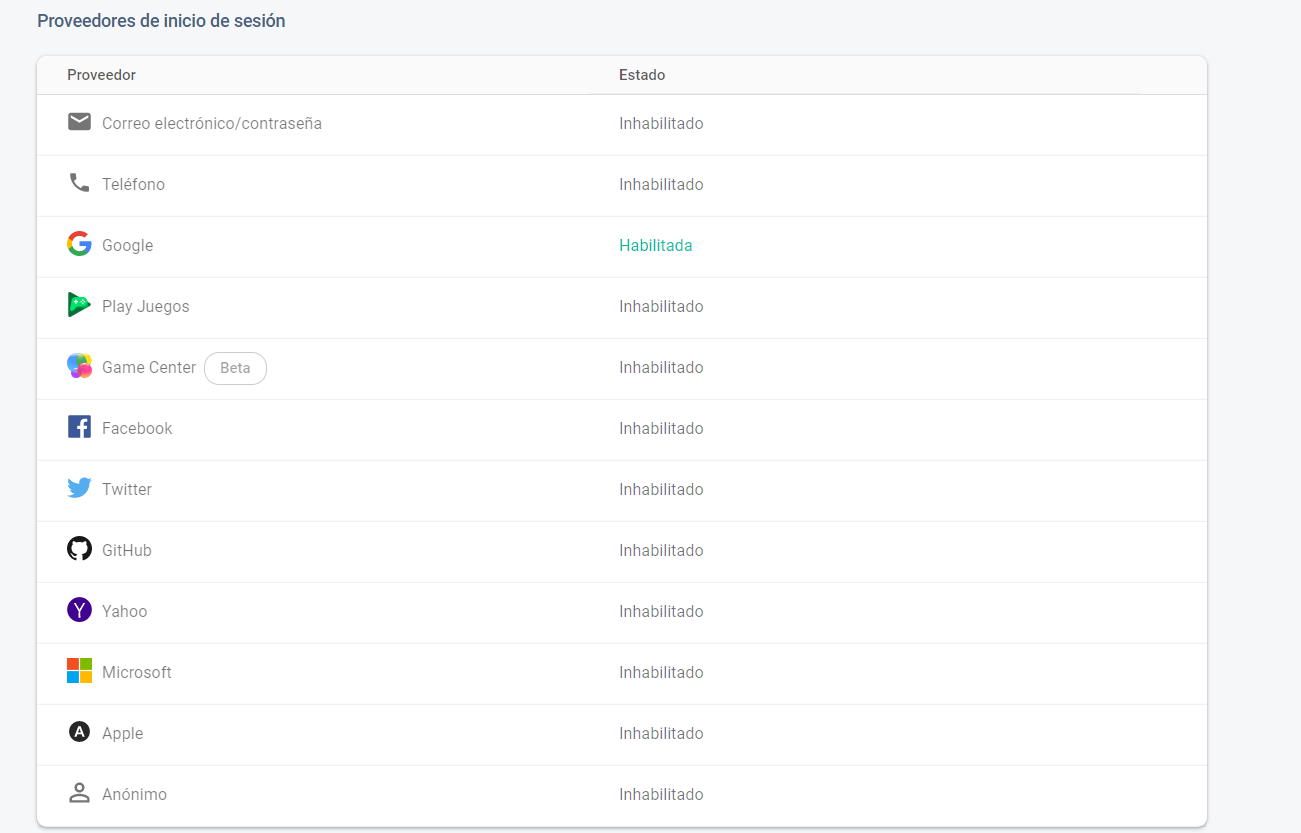
\includegraphics[width=1\textwidth]{teoria/inicio.png}
		\caption{Inicio de sesión}\label{fig:inicio}
	\end{figure}
	\item \textbf{Test lab:} probar la aplicación antes de realizar el despliegue de la misma. También el lanzamiento de pruebas alfa y beta.
	\item \textbf{Remote config:} hacer cambios internos del funcionamiento de la aplicación sin tener que recomplilar o actualizar.
	\item \textbf{Hosting:} servidor donde se puede publicar una página web.
	\item \textbf{Análisis:} mediante las analíticas que ofrece~\ref{fig:numerousers}, sirve como herramienta de toma de decisiones. Pudiendo optimizar a que mercados dirigirse mediante una estrategia de marketing.
	\begin{figure}[H]
		\centering
		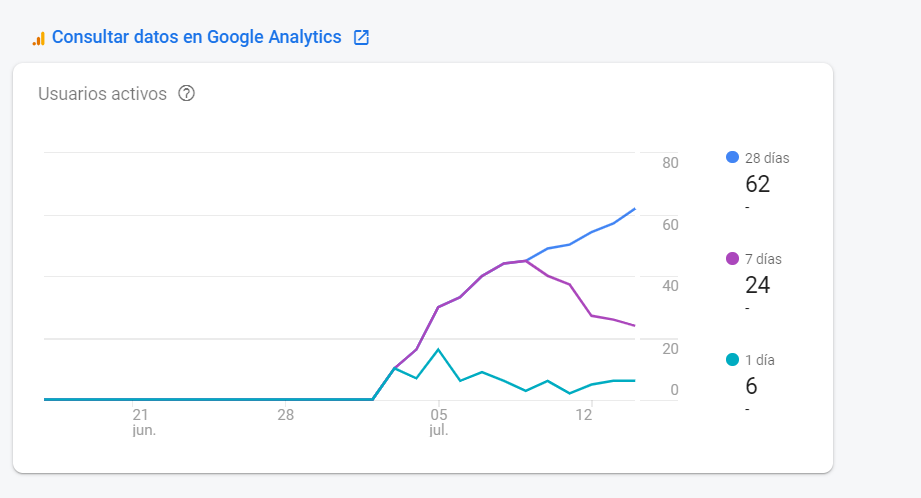
\includegraphics[width=1\textwidth]{teoria/numerousers.png}
		\caption{Ejemplo de Analytics}\label{fig:numerousers}
	\end{figure}
\end{itemize}

\capitulo{4}{Técnicas y herramientas}

Esta parte de la memoria tiene como objetivo presentar las técnicas metodológicas y las herramientas de desarrollo que se han utilizado para llevar a cabo el proyecto. Se comentará de manera breve, las diferentes opciones y la razón porque estás fueron descartadas.

%%%%SISTEMAS OPERATIVOS
\section{Sistema Operativo}

\subsection{Opciones elegidas}

\subsubsection{Microsoft}
~\href{https://www.microsoft.com/es-es}{Microsoft} es el sistema operativo generalista por excelencia. Es de sobra conocido, con sus pros y contras. Fue elegido por comodidad, ya que es el que tengo instalado en mis ordenadores. Además el IDE usado (Visual Studio Code, pág.~\pageref{visual}) para el desarrollo, será de la misma compañía, por lo que hay mayor optimización para este sistema.

\subsubsection{Android}
~\href{https://www.android.com/intl/es_es/}{Android} es un sistema operativo móvil desarrollado por Google. Está basado en el kernel de Linux. Tiene casi toda la cuota de mercado de telefonía. Este se ha usado en mi \emph{smartphone} personal y en las máquinas virtuales, con el fin de probar las aplicaciones en dispositivo físicos y virtualiazdos respectivamente.

\subsection{Alternativas descartadas}

\subsubsection{Ubuntu}
~\href{https://ubuntu.com/}{Ubuntu} es un sistema operativo de código abierto, distribuido bajo una licencia libre. Está basado en Debian, distribución de Linux. Se desarta porque no iba a instalar otro sistema operativo en mis ordenadores personales.


\subsubsection{macOS X}
~\href{https://www.apple.com/es/macos}{macOs} sistema operativo creado por Apple, basado en Unix. Se descarta por que se quiere trabajar con dispositivos Android. Pero en el caso de que se quiera desarrollar para iOS pág.~\pageref{ios}, es indispensable usarlo aquí, porque a la hora de compilar, tira de las librerías internas de este sistema operativo.

\subsubsection{iOS}~\label{ios}
~\href{https://www.apple.com/es/ios}{iOS} sistema operativo para \emph{smartphones} creado por Apple, basado en Unix. Se descarta por que se quiere trabajar con dispositivos Android. Pero en el caso de que se quiera desarrollar para iOS~\pageref{ios}, es indispensable usarlo aquí, porque a la hora de compilar tira de las librerías internas del sistema operativo.

%%CONTROL DE VERSIONES
\section{Control de versiones}

\subsection{Opciones elegidas}

\subsubsection{Git}
~\href{https://git-scm.com//}{Git} es un software de control de versiones, pensado para trabajar con gran cantidad de archivos, con el fin de llevar el registro de los cambios y coordinar a las personas que los comparten. Es gratuito y de código abierto.

Me he decantado por él, porque lo usé durante las prácticas curriculares y extracurriculares de forma intensa, mediante la herramienta Git Bash, ya que mediante comando me siento más cómodo que con una interfaz. Aunque también la dispone mediante el comando \emph{gitk}.

\subsubsection{GitHub}\label{github}
~\href{https://github.com/}{Github} es una plataforma web, recientemente comprada por Microsoft, usada para el control de versiones con las funciones de Git. Entre las diferentes herramientas a destacar: wiki para cada uno de los proyectos, gráficos, funcionalidades de red social, gestor de proyectos, entre otras.

Se escogió esta porque la hemos usado durante el grado y es de sobra conocida. Además ofrece la posibilidad de integración con la herramienta Zenhub~\pageref{zenhub}, para la gestión del proyecto, teniendo las dos cosas centralizadas en el mismo lugar, lo que facilita el proceso de desarrollo.

\subsection{Alternativas descartadas}

\subsubsection{Gitlab}
~\href{https://gitlab.com/}{Gitlab} es igual que Github pero de código abierto ya que tiene licencia MIT. También lo usé en la empresa durante las prácticas pero fue descartado porque me parece de menor calidad. En cuanto a espacio este tiene 10 GB a favor, en contra del 1 GB de Github.

\subsubsection{Bitbucket}
~\href{https://bitbucket.org/product//}{Bitbucket} es otra web más para el control de versiones. Esta enfocado más a la empresa privada, ya que se suele integrar muy bien con otras herramientas de gestión de proyectos. Se descarto por el poco uso que he tenido con este.

\subsubsection{Extensiones Visual Studio Code}
Hay una gran cantidad de herramientas para el control de versiones en la tienda de este editor de código, puede ser práctico, pero las interfaces pueden ser liosas. Por eso me gusta más mediante comando, descartando rápidamente esta opción.

%%% GESTION DE PROYECTOS
\section{Gestión de proyecto}

\subsection{Opción elegida}

\subsubsection{Zenhub}\label{zenhub}
~\href{https://bitbucket.org/product//}{Zenhub} es una herramienta de gestión de proyectos, que viene por defecto integrada en Github, pág.~\pageref{github}, lo que implica a usarla sin pensarlo mucho. En mi caso lo que más usé fue el tablero de \emph{kanban} donde poder ver las \emph{issues} que me planificaba para cada \emph{sprint}. Ofrece diferentes tipos de gráficos, el que mejor se encajaba a la planificación fue de \emph{burndown}, ya que me permite ver lo ideal del proyecto y la progresión que llevo. No me gustó que las tareas las cierra por días en vez de por horas.

\begin{figure}[h]
	\centering
	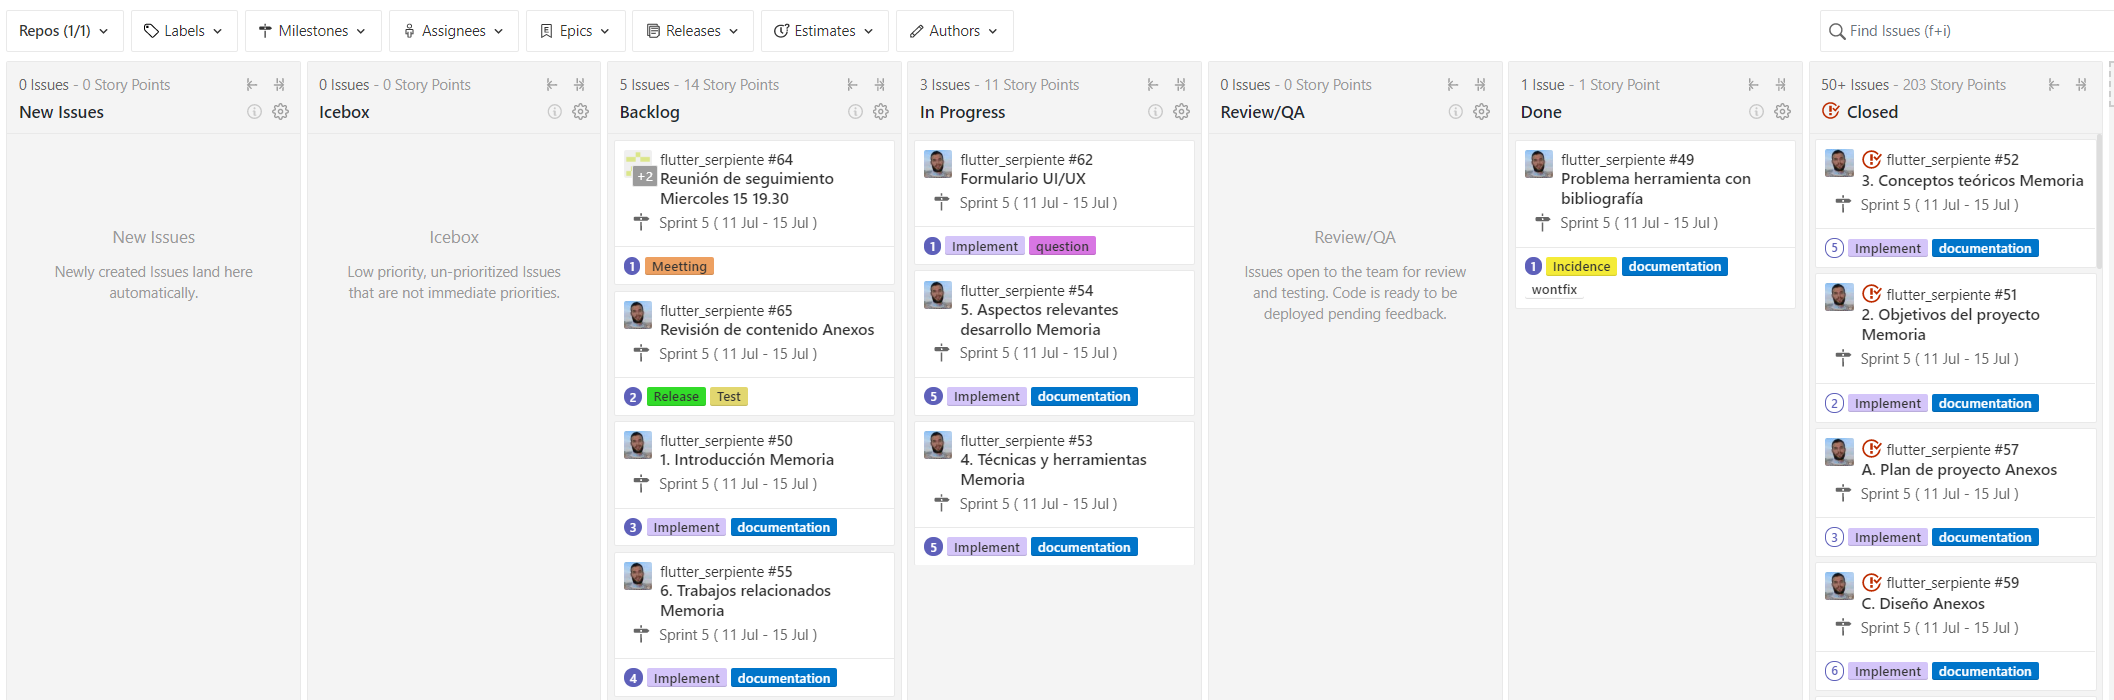
\includegraphics[width=1\textwidth]{teoria/kanban.png}
	\caption{Herramienta Zenhub}\label{fig:zenhub}
\end{figure}

\subsection{Alternativas descartadas}

\subsubsection{Jira}
~\href{https://www.atlassian.com/es/software/jira}{Jira} es una herramienta web propietaria, para el control, seguimiento de errores e incidencias, dentro de la gestión de proyectos. La conozco porque la usé durante las prácticas curriculares, me gustaba mucho, pero no me parece cómoda para lo que quería hacer. Ya que esta herramienta esta orientada en la mejora de procesos en la empresa, que al desarrollo de software.

\subsubsection{Trello}
~\href{https://trello.com/es}{Trello} es una herramienta de gestión de proyectos, con interfaz móvil y web. Usa el sistema kanban como Zenhub~\pageref{zenhub} y tiene integración con Github~\pageref{github}, pero me parece que no encaja en proyectos unipersonales, como era mi caso. Ya que el enfoque es más colaborativo, con grandes grupos de trabajo, donde es necesario compartir documentos con los requisitos, etc ...

%%% ENTORNOS DE PROGRAMACION
\section{Entorno de desarrollo integrado (IDE)}

\subsection{Opción elegida}

\subsubsection{Visual Studio Code}~\label{visual}
~\href{https://code.visualstudio.com/}{Visual Studio Code} es un editor de código fuente desarrollado por Microsoft, cuya licencia es MIT. Esta es totalmente gratuita, con una cantidad enorme de extensiones o \emph{pluggins}, que minimizan esfuerzos, además de la integración con git, que permite ver los cambios en tiempo real. 

Esta facilidad de uso hicieron que me decantase por él.

\subsection{Alternativas descartadas}

\subsubsection{Android Studio}\label{androidstudio}
~\href{https://developer.android.com/studio}{Android Studio} es la herramienta oficial de desarrollo de aplicaciones móviles para el sistema operativo Android. La licencia es Apache 2.0. y sustituye a Eclipse pág.~\pageref{eclipse} como el entorno de desarrollo preferido por Google.

Este IDE se descarta para la creación de código, pero no para las máquinas virtuales.

\subsubsection{Eclipse}~\label{eclipse}
~\href{https://www.eclipse.org/}{Eclipse} es la plataforma software compuesta de varias herramientas de programación de código abierto. Se descartó por ser un IDE no recomendado por parte de Google. Además que a mi parecer es algo tosco.

%% MV
\section{Entorno de virtualización}

\subsection{Opción elegida}

\subsubsection{Android Studio}
~\href{https://developer.android.com/studio}{Android Studio} pág.~\pageref{androidstudio} fue elegido para el despliegue de la aplicación en las máquinas virtuales que ofrece este IDE. Es eficiente y simple, centrado en Android. La creación de las VM es muy cómoda, ya que tiene todo integrado, (con cuatro clicks de ratón se puede lanzar una).

Sumado a que algunas herramientas de Visual Studio Code tiran de estas máquinas, hace que sea la opción más recomendable.

\subsection{Alternativas descartadas}

\subsubsection{Virtual Box}
~\href{https://www.virtualbox.org/}{Virtual Box} es un software de virtualización desarrollado por Oracle. Es de sobra conocido, ya que lo hemos usado durante el grado. Puede desplegar Android, pero al no estar integrado en el desarrollo de aplicaciones, se descató.


%% HERRAMIENTAS DE COMUNICACIÓN
\section{Herramientas de comunicación}

\subsection{Opciones elegidas}

\subsubsection{MS Teams}
~\href{https://www.microsoft.com/es-ww/microsoft-365/microsoft-teams/download-app}{Teams} es la herramienta de comunicación y colaboración integrado en el paquete ofimático de \emph{Office} de Microsoft. Se usó esta herramienta porque con la cuenta de la universidad tenemos acceso a ella y mis tutores de proyecto fueron quienes me la propusieron.

\subsubsection{Outlook}
~\href{https://www.microsoft.com/es-es/microsoft-365/outlook/email-and-calendar-software-microsoft-outlook}{Outlook} es una herramienta de Microsoft para la gestión de la información personal, integrado en la \emph{suite} de Microsoft Office. Se ha usado porque la cuenta de la universidad esta integrada con la plataforma.

\subsection{Alternativas descartadas}

\subsubsection{Gmail}
Es un servicio de correo electrónico proporcionado pro Google. Se descarta porque no tiene integración con la plataforma de la universidad de Burgos.

%% Herramientas para latex
\section{Documentación}

\subsection{Opciones elegidas}

\subsubsection{TexStudio}
~\href{https://www.texstudio.org/}{TexStudio} es un editor de Latex de código abierto, licencia GNU, muy similar a texmaker, pág.~\pageref{textmaker}, ya que es un \emph{fork} de este. Lo que hizo decantarme por el fue la corrección ortográfica interactiva y resaltado de la sintaxis.

\subsubsection{Zotero}
~\href{https://www.zotero.org/}{Zotero} es un gestor de referencias bibliográficas, cuya licencia es AGPL, siendo gratuito. Tiene una extensión para el navegador que ayuda mucho.

\subsection{Alternativas descartadas}

\subsubsection{TexMaker}\label{textmaker}
~\href{https://www.xm1math.net/texmaker/}{Texmaker} es un IDE gratuito para escribir documentos en Latex, su licencia es GPL.

\subsubsection{Overleaf}
~\href{https://www.overleaf.com/}{Overleaf} herramienta web para la edición de documentos escritos en Latex. Esta opción fue descartada porque al ser web, no me permite llevar un seguimiento del versionado como lo puedo hacer, si lo tengo en local con git.

\subsubsection{MS Word}
Editor de documentos de Microsoft, muy conocido, dentro del paquete de ofimática. Se descartó porque la universidad ofrece una plantilla en Latex, de gran calidad y que este no permite el control de versiones.

%% Herramientas varias Google chrome
\section{Herramientas}

\subsection{Opción elegida}

\subsubsection{Google Chrome}
Es un navegador web de código cerrado desarrollado por Google, siendo gratuito. Se ha elegido este pro simpleza porque lo llevo usando desde hace muchos años. Fue usado como ``navaja suiza'', ya que es una herramienta de herramientas, que ha sido usado para multitud de cosas, como:

\begin{itemize}
	\item Para descargar programas, paquetes, librerías...
	\item Para la búsqueda de información.
	\item Edición de imágenes.
	\item Generador de iconos usando el servio web ofrecido por: \href{https://romannurik.github.io/AndroidAssetStudio}{romannurik}
	\item Creación de diagramas ofrecido por la web: \href{https://app.creately.com}{creately}
	\item Armonía de color aportado por la web \href{https://color.adobe.com/es/create/color-wheel}{Adobe color}
\end{itemize}

\subsection{Alternativas descartadas}

\subsubsection{Mozilla Firefox}\label{mozilla}
~\href{https://www.mozilla.org/es-ES/firefox/new/}{Mozilla Firefox} es un navegador de código abierto desarrollado para los principales sistemas operativos. No usado.

%%%METODOLOGIAS
\section{Metodologías}

\subsection{Scrum}
Marco de trabajo para el desarrollo ágil de software, implementando una estrategia iterativa incremental, con revisiones y reuniones con los tutores de proyecto cada 5 días.

\subsection{Desarrollo en cascada}
Es un desarrollo en secuencia, es decir, una vez se pasa de etapa, no se puede volver atrás, se divide en \emph{steps} muy diferenciados, que se adapta my bien con las metodologías ágiles. 

\begin{figure}[h]
	\centering
	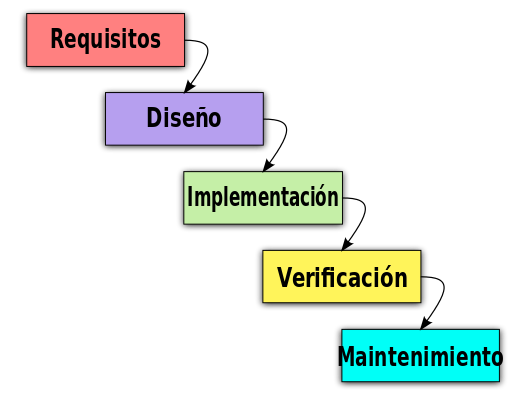
\includegraphics[width=0.8\textwidth]{teoria/cascada.png}
	\caption{Desarrollo en cascada}\label{fig:cascada}
\end{figure}

\subsection{Bolígrafo y cuaderno}
Para mi la parte más importante de toda la gestión del proyecto, reuniones, diseño de las interfaces, control de las horas, planificación, caja negra ... 

Siempre lo he tenido a mi lado como soporte, como se puede ver en la figura~\ref{fig:soporte}:

\begin{figure}[h]
	\centering
	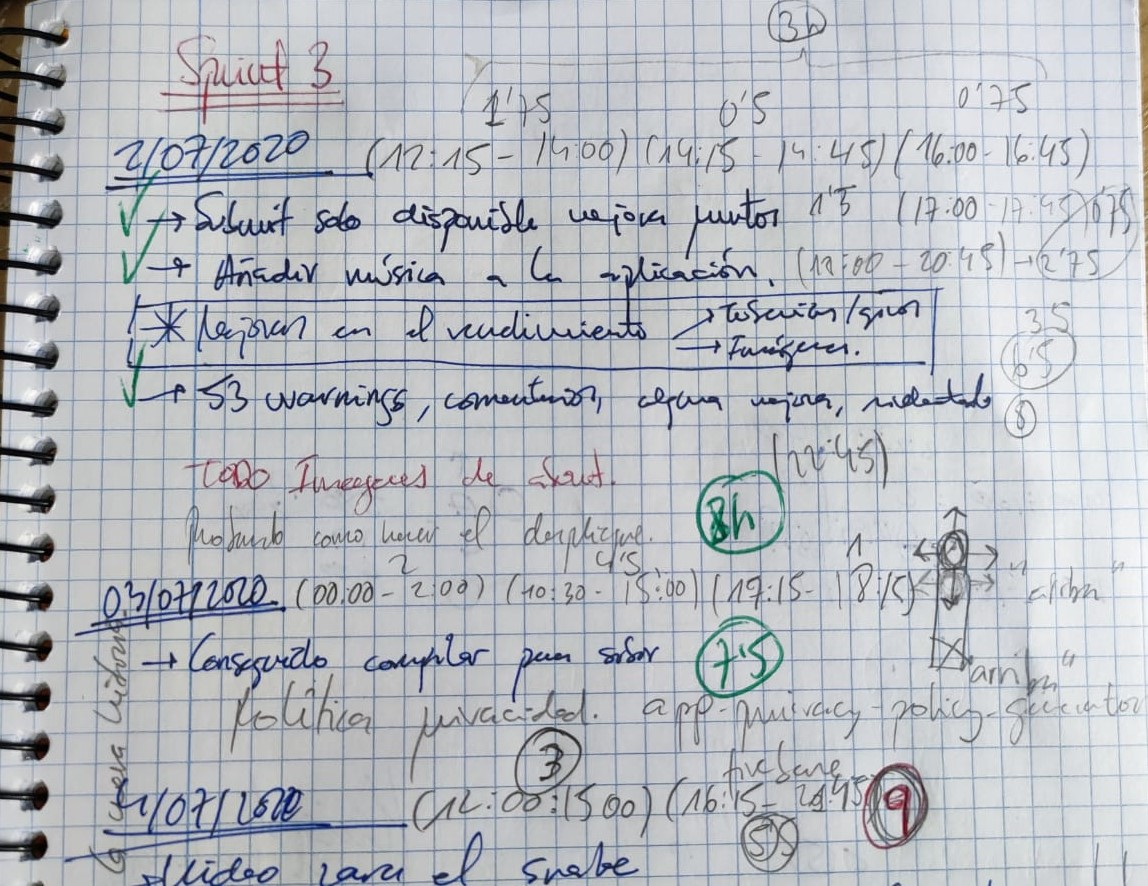
\includegraphics[width=1 \textwidth]{teoria/soporte.jpeg}
	\caption{Cuaderno}\label{fig:soporte}
\end{figure}

\section{Bibliotecas}

\subsection{Material Design}
Es una normativa de diseño o guía de estilos para garantizar una homogeneidad en la visualización dentro de Android. Está desarrollada por Google.

\subsection{Firebase}
Plataforma para el desarrollo de aplicaciones móviles, creada por Google en el 2014. Dispone de una gran cantidad de herramientas de mucha calidad.

\subsection{Play Services }
Librería que permite usar a terceros todas las herramientas ofrecidas por Google.





\capitulo{5}{Aspectos relevantes del desarrollo del proyecto}

En este apartado se recogen los aspectos más importantes o relevantes del desarrollo del proyecto. Desde las decisiones tomadas y las implicaciones que conlleva. Además de los problemas que fueron surgiendo.

\section{Comienzo del trabajo final de grado}
La idea de mi proyecto, surge de la noche a al mañana, porque el problema fue que era el día 20  de junio y no tenía nada para entregar. Esto se debía a que inicialmente iba a hacer otro proyecto basado en \emph{Knime}.

No podía dejar pasar una convocatoria más, debido a que el otro proyecto no me motivaba lo suficiente y con poca documentación al respecto. Aparte no me sentía cómodo con el tema.

Por lo que me decidí estudiar como estaba el mercado de la programación móvil, descubriendo Flutter. Me gustó mucho, todo lo que se comentaba sobre este \emph{Framework}, eran cosas buenas, que era algo nuevo y sobretodo lo que más me decidió a cogerlo, es el respaldo que le daba Google.

Esto se lo comenté a mis tutores de trabajo final de grado, dándome el visto bueno, pero que tenía que trabajar mucho, para llegar a la calidad esperada. Por lo que era un reto enorme al que me enfrentaba, pero como digo, no se pueden dejar pasar las oportunidades, además que por otra parte lo que más me incentivaba, es a la hora de buscar trabajo, no decir que solo me quedaba el TFG. 

Ya que muchas de las empresas me decían que me esperaban a que terminase, para luego cogerme. Y yo no podía esperar, porque si no hacía el TFG, debía de trabajar para no tener que pensar en esto. Por lo que me encontraba entre la ``espada y la pared''.

Por lo que me siento muy agradecido con mis tutores, por haberme dejado cambiar de proyecto, por animarme a conseguirlo, por el feedback constante y darme el soporte necesario.

Finalmente hice un curso en ~\href{https://www.udemy.com/course/flutter-primeros-pasos/}{Udemy}, de unas 40 horas en dos días y medio, para conocer los elementos más básicos, ya que empezaba con los conocimientos que aporta la carrera nada más.

\section{Flutter es asíncrono}
Uno de los mayores retos cuando empiezas a trabajar con este \emph{framework} (ya que en el curso que hice ni se tocan prácticamente), es que se trabaja de manera asíncrona.

Es decir, todo la aplicación se ejecuta en un único hilo, por lo que si un bloque de código se queda congelado, se cuelga todo. Entonces surgen las operaciones asíncronas, que permiten crear funciones o fragmentos de código que no detengan la aplicación entera. Ya que para algunas situaciones es necesario quedarse a la espera como puede ser la llegada de datos de un servidor muy lejano, por lo que no se puede dar al cliente la sensación de que la aplicación se a \emph{freezeado}.

Dentro de Dart son los llamados Future<Object>. Básicamente son tareas que se quedan a la espera, con el fin de que se las devuelva el objeto pedido. Un ejemplo de esto lo podemos ver en~\ref{fig:future}.

\begin{figure}[H]
	\centering
	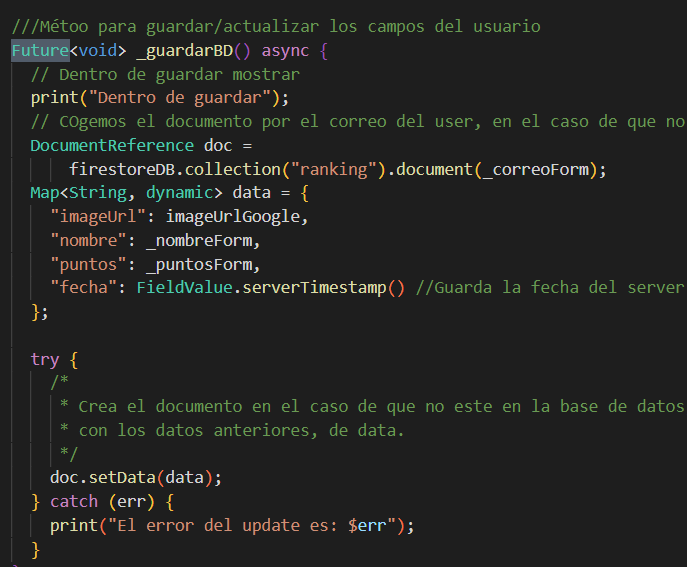
\includegraphics[width=1\textwidth]{teoria/future.png}
	\caption{Ejemplo de Future}\label{fig:future}
\end{figure}

Para ello tenemos que declarar las funciones que son asíncronas con la palabra reservada \emph{async}, de tal manera que devolverá los resultados en un tiempo x.

Cuando realicemos la llamada a estas indicaremos que se queden a la espera de respuesta con \emph{await}.

Pero podemos encontrarnos con otros objetos que también manejan tareas futuras que son los Streams. Haciendo que la aplicación de flutter sea reactiva, como es el caso del cuatro en raya o el ranking.

Estos se definen en un lugar, cogen datos de otro lugar y se queda a la escucha de que se produzcan cambios. En el caso de disparen esos cambios, el Stream se encargará de rediseñar la interfaz del usuario o de actualizar la variables, según el caso.

%\section{Nuevas formas de hacer if}
%Desconocía totalmente esta nueva forma de hacer los condicionales, ya que deja un código más limpio, que ocupa menos líneas e intuitivo. Un ejemplo de esto se puede ver en la imagen siguiente~\ref{fig:nuevoif}:
%
%\begin{figure}[H]
%	\centering
%	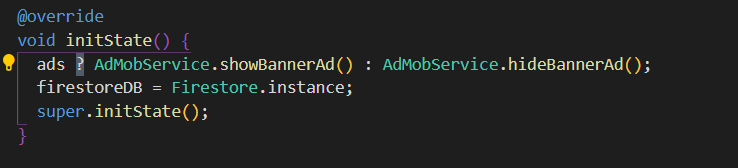
\includegraphics[width=1\textwidth]{teoria/nuevoif.png}
%	\caption{Nuevas formas if}\label{fig:nuevoif}
%\end{figure}

\section{Play Store}
Uno de los problemas encontrados fue a la hora de tener que generar las claves de seguridad, para que la aplicación se pueda subir a la tienda y que ciertos de los servicios estén operativos.

La incidencia estaba que no estaba generando una clave para \emph{debug} y no para \emph{release}, imposiblitando la subida.

Esto era debido a que en la documentación de Flutter siempre se realiza para el modo de test. Luego otra de las cosas a vigilar, es la ruta en la que dejamos la clave y la configuración de algunos ficheros, como los .gradle o el manifest.

Es muy importante tener la clave bien guardada porque en el caso de que se pierda, vamos a tener que volver a realizar el proceso desde cero y es algo tedioso.

\section{AdMob}
Otro de los problemas que he tenido es que a la hora de mostrar los anuncios en la aplicación, no me deja usar los que no son test. He revisado cada uno de los Ids~\ref{fig:idbanner}, pero nada.

\begin{figure}[H]
	\centering
	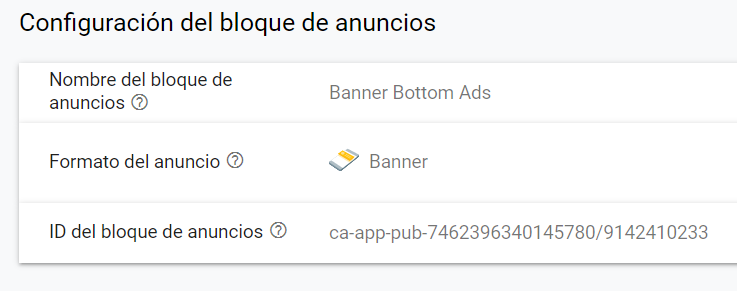
\includegraphics[width=1\textwidth]{teoria/idbanner.png}
	\caption{Banner}\label{fig:idbanner}
\end{figure}

Y las métricas de usuario si que funcionan~\ref{fig:metricas}, por lo que la instancia de adMob es la correcta.

\begin{figure}[H]
	\centering
	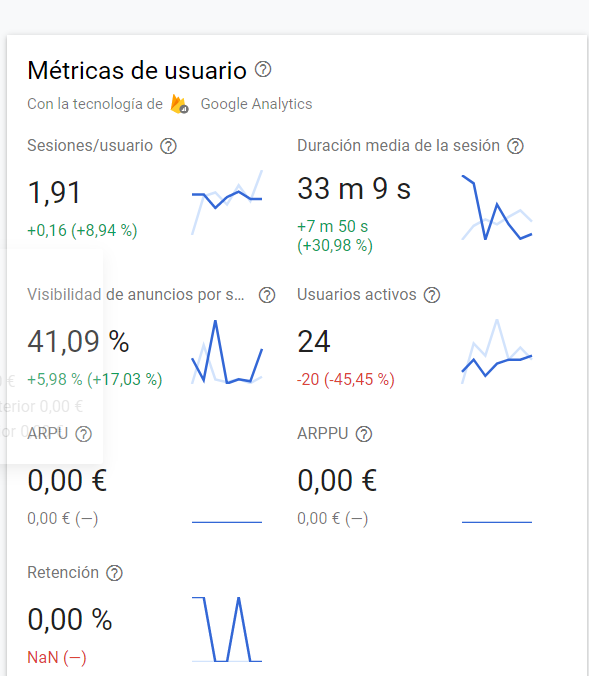
\includegraphics[height=0.8\textwidth]{teoria/metricas.png}
	\caption{Métricas usuarios}\label{fig:metricas}
\end{figure}

Tras investigar y realizar gran cantidad de pruebas creo que el problema puede estar en que no tengo métodos de cobro de ingresos. Por lo tanto la propia Google ni se molesta en poner anuncios. Pero es que la propia consola web de admob, no me deja introducir un método de pago, como se puede ver en la imagen~\ref{fig:pagos}:

\begin{figure}[H]
	\centering
	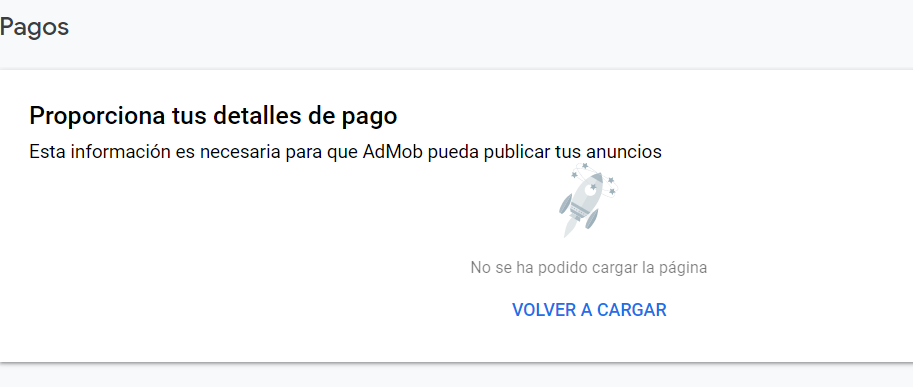
\includegraphics[width=1\textwidth]{teoria/pagos.png}
	\caption{Pagos adMob no van}\label{fig:pagos}
\end{figure}




\capitulo{6}{Trabajos relacionados}

Esta herramienta es muy novedosa, Google la presentó en el 2018, por lo que lleva únicamente dos años en el mercado.

La documentación es escasa y mayoritariamente escrita en inglés. Cada vez hay más información, cursos, y foros al respecto. Entiendo que esto se debe a que Google está apostando fuerte por este lenguaje, ya que ellos son sus creadores.

No me he basado en trabajos anteriores, pero si que he buscado mucha información y me he documentado al respecto. Algunos de los lugares donde he recabado la información son:


\begin{itemize}
	\item Flutter sdk, donde está toda la documentación oficial~\href{https://flutter.dev/}{web}.
	\item Canal oficial de  ~\href{https://www.youtube.com/watch?v=ukLBCRBlIkk&list=PLjxrf2q8roU1kMpfyJ4EY0pID2oRHtvGm}{flutter} en youtube, donde se comenta el Widget de la semana.
	\item Todo lo referente a~\href{https://api.dart.dev/stable/2.8.4/index.html}{dart}.
	\item Canal de youtube sobre ~\href{https://www.youtube.com/channel/UCP4bf6IHJJQehibu6ai__cg}{firebase}.
\end{itemize}
\capitulo{7}{Conclusiones y Líneas de trabajo futuras}

En este apéndice se expone las conclusiones tras la finalización del proyecto final de grado, así como todas las posibles ideas o líneas de trabajo futuras, con el fin de que el proyecto mantenga una continuidad.

\section{Conclusiones}

\begin{itemize}
	\item El objetivo general del proyecto se ha cumplido, ya que todos los requisitos funcionales, como los no funcionales, fueron realizados de manera satisfactoria. Aunque es revisable la mejora de ciertos aspectos, como el diseño de algunas ventanas de la aplicación.
		
	\item Todo el proceso que engloba crear una aplicación, desde la adquisición de los conocimientos, el desarrollo, el diseño, revisiones de producto, la planificación, hasta el despliegue final. 
	
	Indica que se han tocado la mayoría de los conocimientos adquiridos durante el grado, pero que aún así es necesario el constante avance formativo.
	
	\item Adquirir los conocimientos necesarios para la creación de una aplicación en Flutter, ya que es un SDK de gran versatilidad, permitiendo hacer aplicaciones en un tiempo menor.
	
	 Aprender también las herramientas que ofrecidas por parte de Google como Firebase o adMob. \emph{Tools} que desconocía, pero que dan gran valor añadido al producto final.
	
	\item Durante todo el proyecto se usaron gran variedad de aplicaciones, herramientas o dispositivos que ayudaron a mejorar la calidad, rendimiento y funcionalidad del producto final o de algunos de los procesos intermedios. Esto implica tener que especializarse en cada una de ellas, lo que consume recursos temporales.
	
	Pero a la larga este conocimiento aprendido ayudará a tener mejores productos en el futuro.
	
	\item Lidiar con gran incertidumbre, esto se debe que a la hora de planificar es difícil estimar correctamente las horas. Lo que en próximos proyectos puede ser una complicación. Por lo que es una cosa que tengo que mejorar.
	
	Es de gran importancia ajustarse lo máximo posible a la realidad y no pecar de pesimista como es mi caso, ya que planifico más horas de las que luego realmente se invierten.
	
	\item La investigación como parte fundamental a la hora de añadir nuevas funcionalidades al producto como el \emph{sign in} de la aplicación o la publicidad, entre otras.
	
\end{itemize}

En definitiva, personalmente estoy muy contento de haber trabajado duro y haber conseguido una aplicación, ya que desconocía la programación en Android, lo que me ha hecho crecer como persona, pero sobretodo en el ámbito profesional.


\section{Líneas de trabajo futuras}


\begin{itemize}
\item La idea es que la aplicación retenga el mayor tiempo posible a los usuarios para publicidad. Para ello la biblioteca de juegos tiene que seguir creciendo. 

Estos nuevos juegos, se deben de planificar en base a la publicidad para sacar el mayor retorno económico.

\item Internacionalización de la aplicación, para estar disponible en un mayor número de países, de tal manera que el mercado que abarque sea más amplio.

\item Integración de test automáticos como de nuevas metodologías de desarrollo dirigido por test (TDD). Esto mejoraría sustancialmente el rendimiento del programador.

\item Estudio de nuevas herramientas o frameworks destinados a la creación de videojuegos. De tal forma que se pueda migrar los dos juegos actuales, con el fin de ganar un mayor rendimiento.

\item Añadir una inteligencia artificial al juego del cuatro en raya, de tal manera que no solo se pueda jugar online, si no contra la CPU. Como idea esta podría integrar tres niveles de complejidad: facíl, medio y experto. Dentro de la propia Firebase de Google tenemos herramientas de \emph{Cloud computing}, como el \emph{ML kit (Machine learning kit)}. 

Este kit tiene herramientas muy conocidas de Google como puede ser el reconocimiento de texto, etiquetado de las imágenes o detección de las caras, pero se pueden añadir nuestro propios modelos.

\item Realizar el despligue de la aplicación en la tienda de Apple \emph{App Store}, para dispositivos iOS. Y la creación de un hosting donde podamos alojar la aplicación web.
	
\item Integración y exploración de las herramientas de videojuegos como \emph{Play juegos} de Google y la de Apple con su \emph{Game Center}. Esto podría permitirnos las compras in-app.

\item Implementación de algún juego de realidad aumentada con la integración de la publicidad también.
\end{itemize}


\bibliography{bibliografia}
\bibliographystyle{plainnat}

\newenvironment{bottompar}{\par\vspace*{\fill}}{\clearpage}

\begin{bottompar}
\begin{figure}[H]
	\centering
	\includegraphics[width=2cm]{ccby}
\end{figure}


\begin{center}
Este obra está bajo una licencia Creative Commons Reconocimiento 4.0 Internacional
(\href{https://creativecommons.org/licenses/by/4.0/}{CC-BY-4.0}).
\end{center}
\end{bottompar}

\end{document}